\documentclass[main.tex]{subfiles}
\begin{document}


\section{Потеря информации}\label{ch7}

Гравитация не единственное усовершенствование, которое может привести к лучшим моделям. Может быть полезна еще одна интересная модификация, связанная с предыдущей. Это потери информации [9, 108].

\subsection{Зубчатые колеса с потерей информации}\label{ch7.1}

Давайте вернемся к модели зубчатого колеса, обсуждаемой в разд. \ref{2.2}. Самый обобщенный автомат может обладать такой особенностью, что два или более разных начальных состояния превращаются в одно и то же конечное состояние. Например, у нас может быть следующий закон эволюции, включающий 5 состояний:

\begin{equation}\label{7.1}
	(4) \rightarrow (5) \rightarrow (1) \rightarrow (2) \rightarrow (3) \rightarrow (1)
\end{equation}
                                                                                 
Диаграмма для этого закона является обобщением рис. \ref{i2.1}, теперь показанным на рис. \ref{i7.1}. Мы видим, что в этом примере состояние $3$ и состояние $5$ переходят в состояние $1$.

\begin{figure}[ht]
\begin{center}
\scalebox{0.4}{
   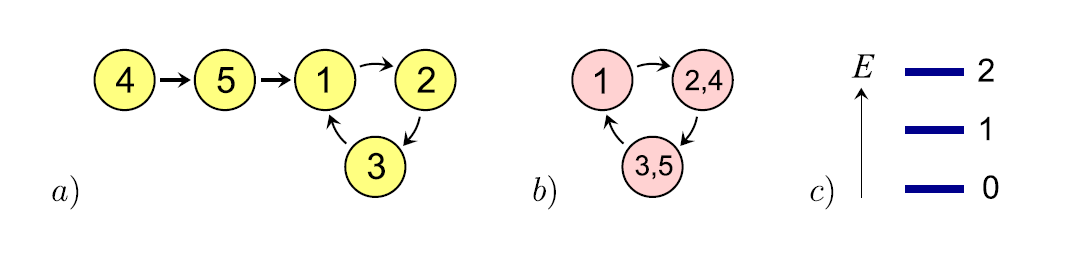
\includegraphics{images/img_7_1.png}
}
\caption{
\label{i7.1}\textbf{a} Простая модель пятиклеточного автомата с информационными потерями \textbf{b} Его три класса эквивалентности \textbf{c} Его три энергетических уровня}
\end {center}
\end {figure}

На первый взгляд можно было бы выбрать в качестве оператора эволюции следующий оператор:

\begin{equation}\label{7.2}
	U(\delta t) \stackrel{?}{=}\left(\begin{array}{ccccc}{0} & {0} & {1} & {0} & {1} \\ {1} & {0} & {0} & {0} & {0} \\ {0} & {1} & {0} & {0} & {0} \\ {0} & {0} & {0} & {0} & {0} \\ {0} & {0} & {0} & {1} & {0}\end{array}\right)
\end{equation}

Тем не менее, поскольку есть два состояния, которые переходят в состояние $ 1$, тогда как нет ни одного, которое превращается в состояние $ 4$, эта матрица не является унитарной, и ее нельзя записать как экспоненту с произведением $-i$ и гамильтониана в показателе.

Можно подумать о внесении крошечных модификаций в оператор эволюции \ref{7.2}, поскольку только бесконечно малые изменения помогут в том, чтобы найти некоторый (не эрмитовый) гамильтониан, который пойдет в показатель экспоненты. Оказывается, это не такая уж и хорошая идея. Лучше детальней разобрать физику таких моделей. Состояния $ 4$ и $ 5$ если и будут реализованы, то только один раз. Как только мы попадаем в цикл, то мы остаемся там. Поэтому имеет смысл просто удалить эти два ложных состояния.

Но тогда возникает проблема: на практике может быть довольно трудно решить, какие состояния находятся в замкнутом цикле, а какие происходят из состояния без прошлого («райские сады»). Здесь это последовательность $4$, $5$ но во многих более реалистичных примерах райские сады будут очень далеко в прошлом, и их будет трудно отследить. Вместо этого мы предлагаем ввести концепцию классов информационной эквивалентности:

  
\textit{Два состояния (a) и (b) в момент времени $t_0$ эквивалентны, если существует время $t_1> t_0$ такое, что в момент времени $t_1$ состояния (a) и (b) перешли в одно и то же состояние (c).}
  

Это определение отправляет состояния $ 5$ и $ 3$ в нашем примере в один класс эквивалентности, также как и $ 4$ и $ 2$. В нашем примере всего 3 класса эквивалентности, и развитие этих классов обуславливается унитарной эволюционной матрицей, поскольку по своей конструкции их эволюция обратима во времени. Классы информационной эквивалентности покажут некоторое сходство с классами калибровочной эквивалентности, и они вполне могут быть довольно большими. Кроме того, понятие локальности будет немного сложнее для понимания, поскольку состояния, которые локально выглядят совершенно по-разному, могут, тем не менее, принадлежать к одному и тому же классу. Конечно, оригинальная базовая классическая модель все еще может быть полностью локальной. Наш любимый пример - игра жизни Конвея [39, 40] с рандомными начальными условиями: произвольная конфигурация единиц и нулей, эволюционирует в соответствии с некоторыми специально выбранными законами эволюции, см. Разд. \ref{ch1.4}. Закон не обратим во времени, и информация теряется в больших масштабах. Следовательно, все классы эквивалентности очень большие, а также общее число классов эквивалентности довольно велико, и модель физически нетривиальна. Пример более общей модели с потерей информации приведен в общих чертах на рис. \ref{i7.2}. Мы видим много классов эквивалентности, каждый из которых может содержать переменные числа членов.

\begin{figure}[ht] % вставляем рисунок
\begin{center}
\scalebox{0.4}{
   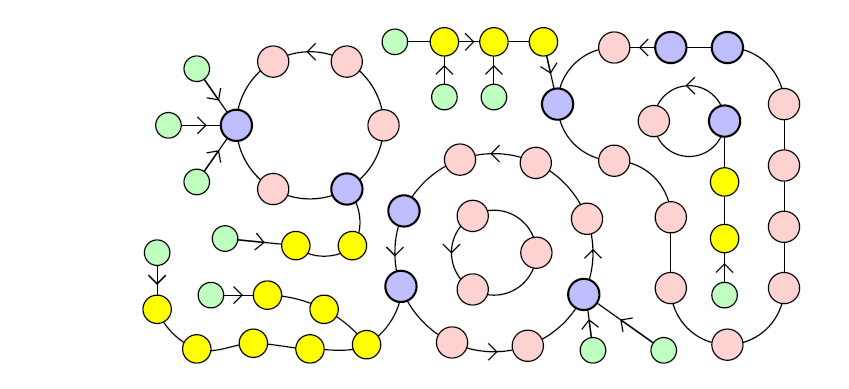
\includegraphics{images/img_7_2.png}
}
\caption{
\label{i7.2} Пример более общей конечной детерминированной необратимой по времени модели. Розовые и синие точки представляют классы эквивалентности. Зеленые точки: «райские сады». Синие: классы эквивалентности, которые имеют «места слияния» среди своих членов. Классы информационной эквивалентности и энергетический спектр такие же, как на рис. \ref{i2.2} и \ref{i2.3}}
\end {center}
\end {figure}


Таким образом, мы находим, как модели с потерей информации все еще могут быть связаны с квантовой механикой:

  
\textit{Каждый класс информационной эквивалентности соответствует элементу онтологического базиса в квантовой теории.}
  

Может ли потеря информации быть полезной? Интуитивно, идея может показаться привлекательной. Рассмотрим процесс измерения, где биты информации, которые изначально были свойствами отдельных частиц, превращаются в макроскопические наблюдаемые. Можно считать, что прошло достаточно времени, и все слияния, которые могут произойти, уже произошли. Другими словами, классические состояния явно представлены по классам эквивалентности. Однако, когда мы все еще имели дело с отдельными кубитами, слияния еще не произошло, и классы эквивалентности могут образовывать очень сложные, в некотором смысле «запутанные», наборы состояний. Локальность в таком случае трудно включить в квантовое описание, поэтому в этих моделях может быть проще ожидать некоторые довольно специфические особенности в отношении локальности - возможно, это именно то, что нам нужно.

Нам также необходимо лучшее понимание черных дыр.  Среди исследователей квантовой гравитации (даже среди приверженцев теории струн)  получает признание идея о том, что черные дыры, испуская излучение Хокинга,  подчиняются квантовой унитарности, а это означает, что гамильтониан все еще является эрмитовым. С другой стороны, классическая черная дыра окружена горизонтом, из которого, кажется, ничто не может вырваться. Теперь мы можем примирить эти явно противоречивые понятия: черная дыра является примером системы с огромными потерями информации на классическом уровне, в то время как квантовая механика ее микросостояний, тем не менее, унитарна. Микро состояния - это не отдельные классические состояния, а просто классы эквивалентности классических состояний. Согласно голографическому принципу, эти классы распределены по всему горизонту таким образом, что у нас есть один бит информации для каждого сегмента области примерно в квадрате длины Планка. Теперь мы интерпретируем это, говоря, что вся информация, проходящая через горизонт, исчезает, за исключением одного бита на единицу площади горизонта.

Мы возвращаемся к излучению Хокинга в секции. \ref{ch9.4}.

\subsection{Обратимость во времени теорий с потерей информации}\label{ch7.2}

Теперь, когда мы занимаемся квантовой механикой, появляется элегантный способ восстановить обратимость времени. Давайте начнем с исходного оператора эволюции $U (\delta t)$, такого как тот, который показан в формуле. (\ref{7.2}). У него нет обратного оператора, но вместо $U^{-1}$ мы могли бы использовать оператор $U^\dagger(\delta t)$, который возвращает нас во времени. Оператор $U^\dagger(\delta t)$, воздействуя на онтологическое состояние $| ont(t_0) \rangle$ в момент времени $t_0$, дает нам аддитивную квантовую суперпозицию всех состояний в прошлом этого состояния во время $t = t_0 - \delta t$. Норма теперь не сохраняется: если в прошлом было N состояний нормализованного состояния $| ont(t_0) \rangle$, то состояние, созданное в момент времени $t_0 - \delta t$, теперь имеет норму $\sqrt{N}$. Если состояние $| ont(t_0) \rangle$ было райским садом, то $U^\dagger | ont(t_0) \rangle = 0$.

Теперь запомните, что всякий раз, когда мы делаем квантовую механику, у нас есть свобода переключаться между базисами, используя унитарные преобразования. Получается, что для любого онтологического оператора эволюции $U_1$, который может быть обобщением уравнения (\ref{7.2}) существует унитарная матрица $X$ со свойством

\begin{equation}\label{7.3}
	U^\dagger_1 X = X U_2
\end{equation}

где $U_2$ опять-таки описывает онтологическую эволюцию с потерей информации. Это нетрудно доказать. Очевидно, что такая матрица $X$ должна существовать, при том, что $U^\dagger_1$ и $U_2$ можно привести в одинаковой нормальной форме. Помимо противоположного временного порядка, $U_1$ и $U_2$ имеют одинаковые классы эквивалентности.

Найти унитарный оператор $X$ не так просто. Мы можем показать, как получить $X$ в очень простом примере. Предположим, что $U_1$ - очень простая матрица $D$ размером $N \times N$ вида
 
\begin{equation}\label{7.4}
	D=\left(\begin{array}{cccc}{1} & {1} & {1} & {\cdots} \\ {0} & {0} & {0} & {} \\ {0} & {0} & {0} & {} \\ {\vdots} & {} & {} & {}\end{array}\right), \quad D^{\dagger}=\left(\begin{array}{cccc}{1} & {0} & {0} & {\cdots} \\ {1} & {0} & {0} \\ {1} & {0} & {0} \\ {\vdots} & {} & {}\end{array}\right)
\end{equation}

так что $D$ имеет $N$ единиц в первом ряду, а остальные строки состоят из нулей. Это просто говорит нам, что $D$ отправляет все состояния $| 1\rangle, ..., | N\rangle $ в одно и то же состояние $| 1\rangle$.

Унитарную матрицу $Y$ подчиняющуюся

\begin{equation}\label{7.5}
	D^\dagger Y = Y D
\end{equation}

можно задать явно:

\begin{equation}\label{7.6}
	Y_{k \ell}=\frac{1}{\sqrt{N}} e^{2 \pi i k \ell / N}
\end{equation}

Этот результат может показаться неожиданным. Интуиция может говорить, что потеря информации сделает наши модели неинвариантными при обращении времени. И все же наш квантово-механический инструмент позволяет нам инвертировать такую модель во времени. «Квантовый наблюдатель» в модели с потерей информации вполне может установить идеальную валидность симметрий, таких как \textit{СРТ}-инвариантность. Это связано с тем, что для квантового наблюдателя преобразования с матрицами $X$ просто представляют переход к другому ортонормированному базису; Матрица $Y$ по существу является матрицей дискретного преобразования Фурье. Обратите внимание, что состояния слияния (см. Рис. \ref{i7.2}) превращаются в райские сады, и наоборот.

\subsection{Стрела времени}\label{ch7.3}

Одной из удивительных вещей, полученных в ходе данного исследования, является новый взгляд на стрелу времени. Локальные законы физики кажутся совершенными в своей обратимости, в то время как классическая физика больших масштабов не обратима во времени вовсе. Разве это не противоречит принципу редукции? Если крупномасштабная физика может быть выведена из мелкомасштабной физики, то как мы можем сделать вывод, что второй закон термодинамики диктует, что энтропия замкнутой системы может только увеличиваться и никогда не уменьшаться?

Большинство физиков не очень обеспокоены этим любопытным фактом. В прошлом  автор всегда объяснял «стрелу времени», тем  что  мелкомасштабные законы Природы обратимы во времени, а граничные условия нет: состояние вселенной было продиктовано в момент времени t = 0 (Большой Взрыв). Энтропия исходного состояния была очень мала, вероятно, просто равна нулю. Для Большого Апокалипсиса не может быть граничного условия, $t = t_\infty$. Итак, существует асимметрия во времени, и тут ничего не поделаешь. Но некоторые исследователи не удовлетворены таким простым ответом.

Теперь у нас есть более радикальная идея: микроскопические законы могут вообще не быть обратимыми во времени. Классической теории, лежащей в основе квантовой механики, не должно быть, см. Разд. \ref{ch7.1}. Затем в разделе \ref{ch7.2}, мы показали, что, даже если классические уравнения характеризуются потерей информации в большом масштабе - так что сохраняются только крошечные доли информации - появляющиеся квантово-механические законы продолжают быть точно обратимыми во времени, так что, пока мы придерживаемся описание вещей в терминах гильбертова пространства, мы не можем понять источник асимметрии времени.

Напротив, классические онтологические состояния очень асимметричны во времени, потому что, как мы заявляли, они напрямую связаны с основными классическими степенями свободы.

Все это может сделать потерю информации приемлемой в теориях, лежащих в основе квантовой теории. Отметим, кроме того, что наше различие онтологических состояний должно быть сохранено, потому что классические состояния являются онтологическими. Онтологические состояния не превращаются в онтологические состояния при обращении времени, поскольку операторы преобразования $X$ и $Y$ включают квантовые суперпозиции. Напротив, шаблоны превращаются в шаблоны. Это автоматически означает, что классические состояния (см. Раздел \ref{ch4.2}) не являются инвариантными относительно обращения времени. Действительно, они не выглядят инвариантными при обращении времени, поскольку классические состояния обычно подчиняются правилам термодинамики.
Квантовые уравнения нашего мира инвариантны (точнее: ковариантны) при обращении времени, но ни субмикроскопический мир, где царят самые фундаментальные законы природы, ни классический мир не допускают обращения времени.

Наше представление о потере информации может иметь еще одно преимущество: два состояния могут находиться в одном классе эквивалентности, даже если мы не можем проследить эволюцию очень далеко назад во времени. На практике можно заподозрить, что вероятность того, что два разных состояния действительно будут в одном классе эквивалентности, со временем быстро уменьшится; эти состояния будут показывать все больше и больше различий в разных местах. Это означает, что мы ожидаем, что физически релевантные классы эквивалентности будут связаны преобразованиями, которые все еще выглядят локально в масштабе частиц, которые в настоящее время могут быть исследованы экспериментально. Это подводит нас к наблюдению, что классы локальной калибровочной эквивалентности могут фактически отождествляться с классами информационной эквивалентности. Это еще (далеко) за пределами наших нынешних математических навыков, чтобы исследовать эту возможность более подробно.

Наконец, обратите внимание, что классы инфоэквивалентности могут вызывать тонкий вид кажущейся нелокальности в нашей эффективной квантовой теории, вид нелокальности, который может помочь принять нарушение теоремы Белла (раздел \ref{ch3.6}).

Явные модели, которые мы изучали, обычно не имеют потери информации. Это потому, что математика будет намного сложнее; мы просто еще не смогли использовать потерю информации в наших более физически значимых примерах.

\subsection{Потери информации и термодинамика}\label{ch7.4}

Есть еще одна важная новинка, для которой мы допускаем потерю информации, особенно когда это происходит в крупном масштабе (вспоминаем рассмотренные выше черные дыры). Ни оператор $U$, ни $U^\dagger$ сейчас не унитарны. С (\ref{7.4}) можно связать:

\begin{equation}\label{7.7}
	DD^\dagger = N |1\rangle \langle 1|,\quad D^\dagger D= N |e\rangle \langle e|
\end{equation}
                          
где $|e \rangle$ - нормализованное состояние

\begin{equation}\label{7.8}
	|e \rangle = \frac 1 {\sqrt{N}} \left( |1 \rangle + ...X|N \rangle\right)
\end{equation}
           
(которое показывает, что матрица $Y$ здесь должна отображать состояние $|1>$ в состояние $|e \rangle$. Обратите внимание, что $D$ и $D^\dagger$ находятся в одном классе сопряженности). Таким образом, в ходе эволюции состояние $|1\rangle$ может стать более вероятным, тогда как вероятности всех других состояний уменьшаются до нуля. Некоторые классы эквивалентности могут получить  таким образом больше слагаемых, в то время как другие могут оставаться довольно маленькими. В больших системах маловероятно, что вероятность того или иного класса полностью исчезнет, поэтому можно было бы записать амплитуды как

\begin{equation}\label{7.9}
	e^{-iHt - \frac 1 2 \beta E}
\end{equation}
          
где можно испытать искушение интерпретировать величину $E$ как (классическую) энергию, а $\frac 1 2 \beta$ - как мнимую составляющую времени. Этот аспект нашей теории все еще очень умозрительный. Предоставление времени для получения сложных значений может быть важным инструментом, помогающим нам понять причины, по которым энергия имеет нижнюю границу.

\end{document}